\documentclass[10pt,a4paper]{article}

\newcommand{\cvRolle}{Senior C++/Python Backend \& Systems Engineer}
\newcommand{\cvSubheader}{Hochperformante Architekturen $\cdot$ Pragmatischer Problemlöser $\cdot$ Fachexperte}

% ==========================================
% SETTINGS.TEX - ZENTRALE KONFIGURATION
% ==========================================
\usepackage[utf8]{inputenc}
\usepackage[T1]{fontenc}
\usepackage[american]{babel}
\usepackage[top=1.8cm, bottom=1.8cm, left=1.8cm, right=1.8cm]{geometry}
\usepackage{xcolor}
\usepackage{hyperref}
\usepackage{enumitem}
\usepackage{graphicx}
\usepackage{calc}
\usepackage{charter}
\usepackage{microtype}
\usepackage{etoolbox}

% --- DESIGN FARBEN ---
\definecolor{primary}{RGB}{15, 23, 42}      % Deep Slate / Tech Dark
\definecolor{accent}{RGB}{37, 99, 235}     % MP Blue Accent
\definecolor{textgray}{RGB}{51, 65, 85}    % Charcoal Body Text

% --- PERMANENTE ABSENDER-DATEN ---
\newcommand{\meinName}{Markus Gruber, M.Sc.}
\newcommand{\meineStrasse}{Maximilianstraße 55 Stg. B 20}
\newcommand{\meinOrt}{3100 St. Pölten}
\newcommand{\meineEmail}{Markus.Gruber4@gmx.net}
\newcommand{\meineTel}{+43 650 5871145}
\newcommand{\meinLinkedin}{https://www.linkedin.com/in/markus-gruber-70851428/}
\newcommand{\meinGithub}{https://github.com/CodeByMaxx}

% --- ROLLEN-DEFAULTS ---
\providecommand{\cvRolle}{}
\renewcommand{\cvRolle}{AI & Automation Engineer -- M&A Deal Automation}
\providecommand{\cvSubheader}{}
\renewcommand{\cvSubheader}{Python \cdot LLM APIs (OpenAI, Anthropic) \cdot Financial Data Pipelines \cdot Agent Workflows \cdot RAG}

% --- EMPFÄNGER-DATEN ---
\newcommand{\firmenName}{MP Corporate Finance}
\newcommand{\ansprechPartner}{Katharina Schwarzl-Moser (HR Manager)}
\newcommand{\firmenStrasse}{Wien, Österreich}
\newcommand{\firmenOrt}{Wien, Österreich}

% --- INTELLIGENTE ADRESS-AUSGABE (Verhindert doppelte Zeilen, wenn Straße == Ort) ---
\newcommand{\firmenAdresse}{%
    \def\tempStrasse{Wien, Österreich}%
    \def\tempOrt{Wien, Österreich}%
    \ifx\tempStrasse\tempOrt
        \tempOrt%
    \else
        Wien, Österreich \\[0.15em] Wien, Österreich%
    \fi
}

\newcommand{\stellenTitel}{AI & Automation Engineer (f/m/x)}
\newcommand{\referenzNummer}{}

\newcommand{\anrede}{Dear Ms. Schwarzl-Moser,}
\newcommand{\firmenHighlight}{MP Corporate Finance is one of Europe's leading mid-market M&A boutiques, where your AI tools will be deployed on live cross-border transactions from day one.}

% --- HEADER BEFEHL ---
\newcommand{\cvHeader}{%
\begin{center}
    {\Huge\bfseries\color{primary} \meinName}\\[0.1cm]
    {\large\bfseries \cvRolle}\\[0.05cm]
    {\color{accent}\textbf{\cvSubheader}}\\[0.1cm]
    {\small \meinOrt, Austria \quad$\cdot$\quad \meineTel \quad$\cdot$\quad \href{mailto:\meineEmail}{\meineEmail} \quad$\cdot$\quad \href{\meinLinkedin}{LinkedIn} \quad$\cdot$\quad \href{\meinGithub}{GitHub}}
\end{center}
\vspace{0.1cm}
}

% --- BEFEHLE FÜR LEBENSLÄUFE & ANSCHREIBEN ---
\newcommand{\cvsection}[1]{%
    \vspace{0.25cm}%
    {\Large\bfseries\color{primary} #1}\par%
    \vspace{-0.1cm}{\color{primary}\rule{\textwidth}{0.8pt}}\par%
    \vspace{0.15cm}%
}

\newcommand{\daterange}[2]{\hfill{\small #1 -- #2}}

% --- ENGINEERING APPROACH & MINDSET DEFINITION ---
\newcommand{\engineeringApproach}{%
    \cvsection{Engineering Approach \& Mindset}%
    \begin{itemize}[leftmargin=*, itemsep=2pt]%
        \item \textbf{Systematic Problem Solving:} First-principles analytical approach to systematic debugging and stability optimization.%
        \item \textbf{Quality & Efficiency Focus:} Pragmatic engineering mindset balancing rapid deployment with long-term maintainability and high performance.%
        \item \textbf{Cross-Functional Integration:} Acts as the technical glue bridging development, QA, and architecture.%
    \end{itemize}%
}

% --- HYPERREF SETUP ---
\hypersetup{
    colorlinks=true,
    linkcolor=primary,
    urlcolor=primary,
    pdfauthor={\meinName},
    pdftitle={Application Documents - \meinName}
}


\pagestyle{empty}

\begin{document}

\setlength{\parindent}{0pt}
\setlist[itemize]{leftmargin=1.5em, itemsep=0.15em, topsep=0.15em}

\cvHeader

\cvsection{Berufliches Profil}

% --- BILD LINKS, TEXT RECHTS UNTER DER ÜBERSCHRIFT ---
\begin{minipage}[t]{0.22\textwidth}
    \vspace{0pt}
    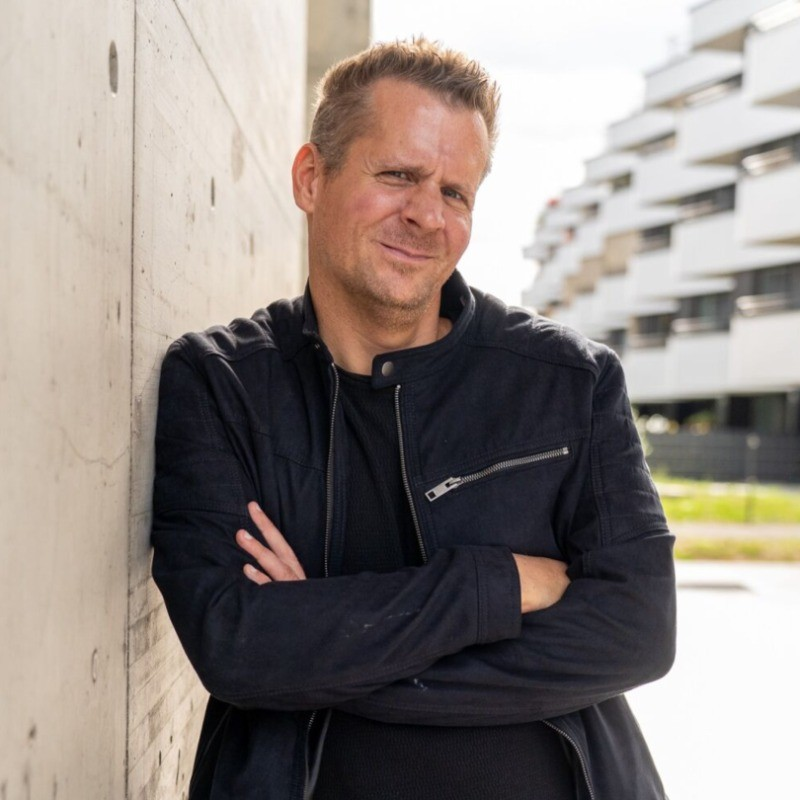
\includegraphics[width=\linewidth, keepaspectratio]{profil.jpeg}
\end{minipage}
\hfill
\begin{minipage}[t]{0.75\textwidth}
    \vspace{0pt}
    Pragmatischer Senior C++/Python Backend \& Systems Engineer mit 9+ Jahren Erfahrung in der Entwicklung von Echtzeit-Pipelines, Cloud-Microservices und hochperformanten Systemen. Inhaber eines M.Sc. in Scientific Computing mit starkem mathematischen Fundament.\\\\[0.1cm]
    Belastbarer Problemlöser zur Behebung kritischer Produktionsengpässe und Speicherlecks. Agiert als effektive Schnittstelle zwischen Entwicklung, QA und Architektur unter Nutzung moderner KI-Tools (Cursor, Copilot).
\end{minipage}

\vspace{0.3cm}

\cvsection{Technisches Profil}

\colorbox{primary!10}{%
\parbox{\dimexpr\textwidth-2\fboxsep\relax}{%
    \vspace{0.10cm}
    \centering
    {\bfseries\color{primary} TECHNISCHE GRUNDLAGEN \& SYSTEMDOMÄNEN\par}
    \vspace{0.08cm}

    \begin{minipage}[t]{0.31\linewidth}
        \raggedright
        \textbf{\color{primary}Kernsysteme \& Engineering}\par
        Modernes C++, C, Python, Bash\\
        Speicheroptimierung \& Refactoring\\
        Multithreading \& Deterministische Systeme
    \end{minipage}
    \hfill
    \begin{minipage}[t]{0.31\linewidth}
        \raggedright
        \textbf{\color{primary}Plattform \& Infrastruktur}\par
        AWS (S3, RDS, EC2) \& Azure\\
        Linux-Ökosystem \& Docker\\
        GitLab CI/CD \& Auto-Test-Pipelines
    \end{minipage}
    \hfill
    \begin{minipage}[t]{0.31\linewidth}
        \raggedright
        \textbf{\color{primary}KI, Daten \& High-Throughput}\par
        RAG-Infrastruktur \& Vektordatenbanken\\
        Verteilte Datenverarbeitung \& REST APIs\\
        CUDA Hardwarebeschleunigung \& Edge GPU
    \end{minipage}

    \vspace{0.08cm}
}%
}

\vspace{0.20cm}
\textbf{\color{primary}TECHNISCHE SPEZIALISIERUNG -- SYSTEMS ENGINEERING}
\begin{itemize}
    \item \textbf{Hochperformante Backend-Architektur:} Modernes C++ Systemdesign, cache-effiziente Datenstrukturen und latenztarme Ausführung in ressourcenkritischen Backends.
    \item \textbf{System-Profiling \& Speicher-Debugging:} Ursachenanalyse von Speicherlecks, Race Conditions und Latenzspitzen zur Maximierung von Laufzeit und Systemstabilität.
    \item \textbf{Daten-Pipelines \& Integrationsinfrastruktur:} Architektur von Datenverarbeitungs- und Integrationspipelines mit hoher Durchsatzrate bei gleichzeitiger Automatisierung der Release-Verifizierung.
\end{itemize}

\cvsection{Berufserfahrung}

\textbf{Mindbreeze GmbH -- Software / Quality Engineer (C++/Python)} \daterange{09/2022}{07/2026}\\
\textit{C++, Python, REST APIs, Linux, Docker, Azure DevOps, Telemetrie \& Performance-Profiling \quad|\quad Team: 6 Ingenieure}
\begin{itemize}
    \item Entwicklung von Python/Bash-Automatisierungsframeworks, wodurch die Release-Verifizierungsdauer von 10 auf 3 Arbeitstage reduziert wurde.
    \item Optimierung leistungskritischer Backend-Komponenten für Enterprise-Architekturen mit verteilter Datenverarbeitung.
    \item Refactoring von Kernmodulen der Suchmaschine und Optimierung der Index-Datenpipelines zur Verbesserung der Abfrageausführung.
    \item Hauptverantwortlicher technischer Problemlöser während der Release-Phasen (Behebung von Memory Leaks und Performance-Problemen in Live-Systemen).
\end{itemize}

\vspace{0.15cm}
\textbf{Untis GmbH -- Software Engineer (C++)} \daterange{02/2022}{06/2022}\\
\textit{C++, System-Refactoring, Performance-Profiling, Core Desktop Module \quad|\quad Team: 10 Ingenieure}
\begin{itemize}
    \item Refactoring von Legacy C++/MFC-Kernmodulen in Visual Studio zum Abbau technischer Schulden, zur Optimierung von Speicherallokationen und zur Behebung von Produktionsabstürzen.
\end{itemize}

\vspace{0.15cm}
\textbf{logi.cals -- Embedded Software Engineer (C/C++)} \daterange{02/2021}{01/2022}\\
\textit{C, C++, Embedded Systems, Sicherheitskritische Architekturen, Deterministische Ausführung \quad|\quad Team: 6 Ingenieure}
\begin{itemize}
    \item Entwicklung deterministischer C/C++-Laufzeitsysteme (Software-SPS) und automatisierter Verifizierungstestsuiten für Sicherheitszertifizierungen auf verschiedenen Hardwareplattformen.
\end{itemize}

\vspace{0.15cm}
\textbf{EYYES -- Software Engineer (C++/Python)} \daterange{04/2017}{12/2020}\\
\textit{C++, Python, Echtzeit-Ausführungspipelines, CUDA, Embedded GPU Edge \quad|\quad Team: 8 Ingenieure}
\begin{itemize}
    \item Entwicklung von Computer Vision- und Deep Learning-Pipelines (Keras, ONNX) für industrielle Kamera-Systeme zur Sicherstellung kontinuierlicher Echtzeit-Leistung auf Edge-Geräten.
    \item Entwicklung latenzarmer C++- und CUDA-Ausführungsroutinen für die Echtzeit-Videostreambearbeitung auf eingebetteten GPU-Edge-Geräten.
    \item Implementierung hardwarenaher Softwarekomponenten in C++ zur Steuerung von Kamerasensoren, Schrittmotoren und SerDes-Schnittstellen.
    \item Optimierung der Erkennungsgenauigkeit durch Training mehrerer TensorFlow-Klassifikatoren auf 99,99\% Präzision mittels hardwarenahem Algorithmentuning und automatisierter Benchmarking-Suiten.
\end{itemize}

\cvsection{Ausgewählte Softwareprojekte}

\begin{itemize}
    \item \textbf{Magnum C++ Game of Life:} Hochperformante C++-Simulation mit Fokus auf Speicherlayout und objektorientiertes Design (\href{\meinGithub}{GitHub}).\\
    \textit{Tech: Modernes C++, Speicherlayout, Optimierung, Grid-Logik}
    \item \textbf{AWS Cloud Deep Learning Pipeline:} MLOps-Pipeline mit automatisierter Datenerfassung und PyTorch-Inferenz (\href{\meinGithub}{GitHub}).\\
    \textit{Tech: AWS, Python, PyTorch, MLOps}
    \item \textbf{Azure AI Document Analyzer \& RAG Infra:} RAG-Processing-Backend auf Azure mit Vektordatenbanken (\href{\meinGithub}{GitHub}).\\
    \textit{Tech: Python, RAG, Vektordatenbanken, REST APIs}
\end{itemize}

\cvsection{Technische Kenntnisse}

\textbf{Sprachen \& Kernkompetenzen:} Modernes C++, C, Python, SQL, Java, Bash, Speichermanagement, Parallele Algorithmen, Scientific Computing.\\[0.05em]
\textbf{ML, KI \& Data Engineering:} PyTorch, TensorFlow, Keras, ONNX, RAG-Infrastruktur, LangChain, LangGraph, PySpark, DuckDB, PostgreSQL, SQLAlchemy, Apache Superset.\\[0.05em]
\textbf{Cloud, Systeme \& Infrastruktur:} Amazon AWS (S3, RDS, EC2), Microsoft Azure, Linux (Ubuntu/Debian), Windows, Docker, Microservices, REST APIs.\\[0.05em]
\textbf{DevOps, QA \& Tools:} GitLab CI/CD, GitHub Actions, Azure DevOps, Git, Telemetrie, Cursor, GitHub Copilot, CUDA, OpenCL, OpenMP, MPI, Embedded GPU Edge.

\cvsection{Ausbildung}

\textbf{M.Sc. Scientific Computing} -- Universität Wien \daterange{10/2013}{06/2017}\\
\textit{Masterarbeit: Silent Data Corruption in FT-GMRES (\href{https://utheses.univie.ac.at/detail/40917/}{Link}, Betreuer: Prof. Dr. W. Gansterer).}

\vspace{0.1cm}
\textbf{B.Sc. Industrial Simulation} -- FH St. Pölten \daterange{09/2010}{06/2013}\\
\textit{Bachelorarbeit: Simulation von Nanokomposit-Materialien (\href{\meinGithub}{Link}, Betreuer: Prof. Dr. T. Schrefl).}

\cvsection{Arbeitsweise \& Ingenieursphilosophie}

\begin{itemize}
    \item \textbf{Systematische Problemlösung:} Analytischer Ansatz zur systematischen Fehlersuche und Optimierung der Systemstabilität.
    \item \textbf{Qualität \& Effizienz:} Pragmatische Denkweise, die schnelle Bereitstellung mit langfristiger Wartbarkeit und hoher Leistung verbindet.
    \item \textbf{Interdisziplinäre Zusammenarbeit:} Versteht sich als technische Schnittstelle zwischen Entwicklung, QA und Architektur.
\end{itemize}

\cvsection{Sprachen \& Arbeitsstatus}

\textbf{Deutsch:} Muttersprache (C2) \quad$\cdot$\quad \textbf{Englisch:} Verhandlungssicher (C1/C2) \quad$\cdot$\quad \textbf{Arbeitserlaubnis:} EU-Bürger / Österreich

\end{document}